\documentclass[11pt,a4paper]{article}
\usepackage[margin=2.5cm]{geometry}
\usepackage{amsmath}
\usepackage{booktabs}
\usepackage{listings}
\usepackage{xcolor}
\usepackage{hyperref}
\usepackage{microtype}
\usepackage{parskip}
\usepackage{caption}
\usepackage{tikz}
\usetikzlibrary{arrows.meta, positioning, shapes.geometric}

\lstset{
  basicstyle=\ttfamily\small,
  keywordstyle=\color{blue!70!black}\bfseries,
  commentstyle=\color{green!50!black},
  stringstyle=\color{red!60!black},
  breaklines=true,
  frame=single,
  numbers=left,
  numberstyle=\tiny\color{gray},
  tabsize=4,
}

\title{\textbf{ImperativeAgentV3: A Deterministic State-Machine Architecture\\
for Multi-Step Banking Customer Service}}
\author{GenAI Project --- SMU IS714}
\date{May 2026}

\begin{document}
\maketitle

\begin{abstract}
We describe ImperativeAgentV3, a deterministic state-machine LLM agent designed for the
$\tau$-Banking benchmark~\cite{tau2bench}. Building on ImperativeAgentV2's eight-phase pipeline,
V3 introduces six structural improvements: an explicit task queue with topological ordering,
state-driven (rather than heuristic) phase transitions, a verification hard gate, a per-tool
retry policy with deterministic escalation, and strict response-type enforcement. These
improvements target the core failure modes of V2: non-deterministic phase transitions under
ambiguous message types, missing enforcement of the verification precondition, uncontrolled
retries on tool failures, and model non-compliance with phase expectations.
\end{abstract}

\tableofcontents
\newpage

% ---------------------------------------------------------------------------
\section{Background}
% ---------------------------------------------------------------------------

\subsection{The $\tau$-Banking Benchmark}

$\tau^2$-Bench~\cite{tau2bench} evaluates LLM agents on realistic customer-service conversations.
The \texttt{banking\_knowledge} domain contains 97 tasks covering account management, credit card
operations, dispute resolution, and product inquiries. Each task specifies a customer intent that
may require up to 18 knowledge-base (KB) documents and an average of 9.52 tool calls to resolve
correctly. Success is measured by $\text{pass}^1$ (fraction of tasks fully resolved in one trial).

\subsection{Declarative vs.\ Imperative Orchestration}

Our project compares two orchestration paradigms:

\begin{description}
  \item[Declarative] The agent's system prompt includes skill files (Markdown documents)
    that describe available actions and constraints. The LLM decides the workflow at runtime.
  \item[Imperative] The agent's code encodes a deterministic finite automaton (DFA) over a
    set of named phases. The LLM executes a scripted goal within the current phase; phase
    transitions are computed deterministically by the agent code.
\end{description}

The imperative design decouples \emph{what to do} (LLM responsibility) from
\emph{when to transition} (code responsibility), reducing the surface area for hallucination
and improving interpretability.

% ---------------------------------------------------------------------------
\section{ImperativeAgentV2: Architecture and Failure Modes}
% ---------------------------------------------------------------------------

\subsection{Phase Sequence}

V2 defines eight phases:
\[
\text{GREETING} \to \text{TRIAGE} \to \text{VERIFICATION} \to \text{PLANNING} \to
\text{EXECUTION} \to \text{CONFIRMATION} \to \text{COMPLETE}
\]
with an \texttt{ADVISORY} branch for informational requests that bypasses verification
and planning.

\subsection{Phase Transition Mechanism}

V2 transitions are driven by \emph{message-type heuristics}: the phase logic inspects
whether the most recent assistant message was a tool call or text, and whether the most
recent tool result succeeded. For example:

\begin{lstlisting}[language=Python, caption={V2 TRIAGE transition logic}]
if current == "TRIAGE":
    last_tool = self._last_tool_name(state)
    if last_tool and last_tool in IDENTIFICATION_TOOLS:
        if self._last_was_successful_tool_result(state):
            return "VERIFICATION"
    ...
\end{lstlisting}

\subsection{Identified Failure Modes}

\begin{enumerate}
  \item \textbf{Heuristic fragility}: message-type heuristics misfire when the model
    returns an unexpected response type (e.g., text when a tool call was expected).
    The phase may stay or advance based on the wrong signal.
  \item \textbf{Missing verification gate}: the transition from TRIAGE to VERIFICATION
    is conditioned on a successful identification tool call, but EXECUTION is never
    re-checked. A bug in PLANNING could allow reaching EXECUTION without verified = True.
  \item \textbf{Uncontrolled tool retries}: repeated failures of the same tool cause
    the agent to loop indefinitely with no upper bound and no escalation path.
  \item \textbf{Implicit task ordering}: the PLANNING phase instructs the LLM to find
    ordering constraints and list tasks in order, but the resulting list is not stored
    in agent state. If the model forgets the plan mid-EXECUTION, ordering is lost.
  \item \textbf{No response-type enforcement}: a model that returns text when a tool
    call is expected (or vice versa) simply receives the wrong phase signal; the agent
    does not actively correct it.
\end{enumerate}

% ---------------------------------------------------------------------------
\section{ImperativeAgentV3: Design}
% ---------------------------------------------------------------------------

\subsection{New State Fields}

V3 extends \texttt{AgentState} (a Pydantic model) with six new fields:

\begin{lstlisting}[language=Python, caption={AgentState v3 additions (src/agents/state.py)}]
# Strategy 3 & 4: explicit boolean gates
user_identified: bool = False
verified: bool = False

# Strategy 1 & 2: explicit task queue
pending_tasks: list[str] = Field(default_factory=list)
completed_tasks: list[str] = Field(default_factory=list)

# Strategy 5: per-tool retry tracking
tool_retry_counts: dict[str, int] = Field(default_factory=dict)

# Strategy 6: response-type violation counter
expect_violation_count: int = 0
\end{lstlisting}

\subsection{New Phase: ESCALATE}

V3 adds an \texttt{ESCALATE} phase that the agent transitions to when any tool's retry
count exceeds its limit. This gives the agent a deterministic exit path for unresolvable
failures rather than looping indefinitely.

\subsection{Phase Graph}

\begin{center}
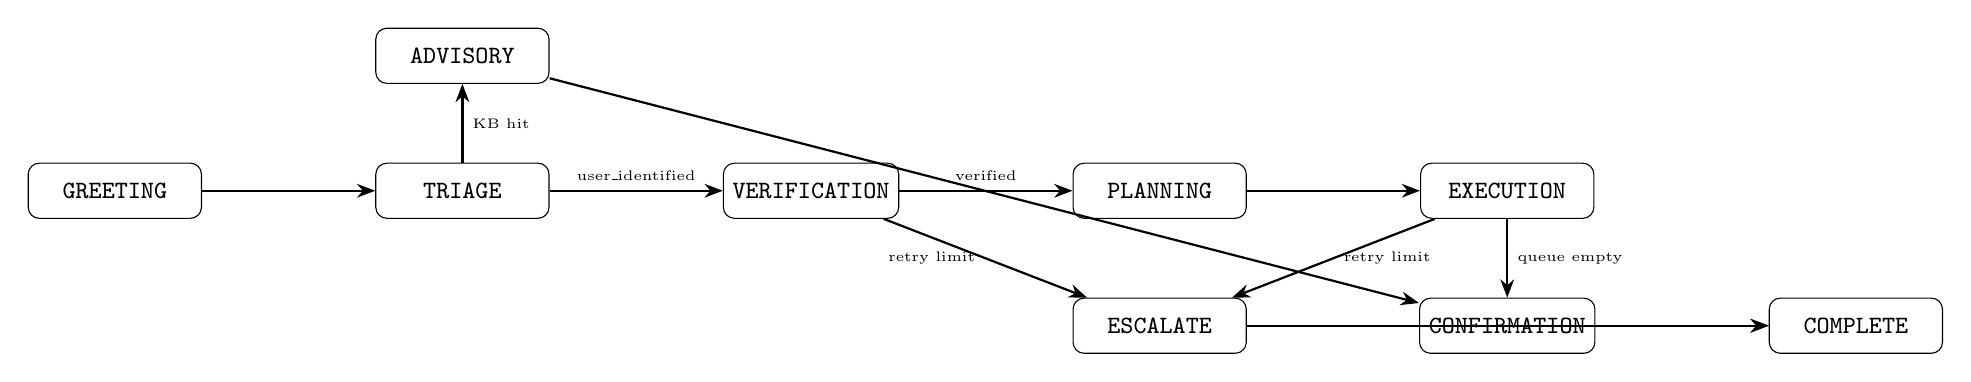
\begin{tikzpicture}[
  node distance=1.5cm and 2.2cm,
  phase/.style={rectangle, draw, rounded corners, minimum width=2.2cm, minimum height=0.7cm,
                font=\small\ttfamily},
  edge/.style={-Stealth, thick},
]
  \node[phase] (G) {GREETING};
  \node[phase, right=of G] (T) {TRIAGE};
  \node[phase, right=of T] (V) {VERIFICATION};
  \node[phase, right=of V] (P) {PLANNING};
  \node[phase, right=of P] (E) {EXECUTION};
  \node[phase, above=1cm of T] (A) {ADVISORY};
  \node[phase, below=1cm of E] (CF) {CONFIRMATION};
  \node[phase, right=of CF] (CO) {COMPLETE};
  \node[phase, below=1cm of P] (ES) {ESCALATE};

  \draw[edge] (G) -- (T);
  \draw[edge] (T) -- (V) node[midway,above,font=\tiny]{user\_identified};
  \draw[edge] (T) -- (A) node[midway,right,font=\tiny]{KB hit};
  \draw[edge] (A) -- (CF);
  \draw[edge] (V) -- (P) node[midway,above,font=\tiny]{verified};
  \draw[edge] (P) -- (E);
  \draw[edge] (E) -- (CF) node[midway,right,font=\tiny]{queue empty};
  \draw[edge] (CF) -- (CO);
  \draw[edge] (V) -- (ES) node[midway,left,font=\tiny]{retry limit};
  \draw[edge] (E) -- (ES) node[midway,right,font=\tiny]{retry limit};
  \draw[edge] (ES) -- (CO);
\end{tikzpicture}
\end{center}

% ---------------------------------------------------------------------------
\section{Six Deterministic Strategies}
% ---------------------------------------------------------------------------

\subsection{Strategy 1: Explicit Task Queue}

The PLANNING phase instructs the model to output its task list in a structured block:

\begin{lstlisting}
TASKS:
1. Request credit limit increase
2. File transaction dispute
END_TASKS
\end{lstlisting}

The agent parses this block at the PLANNING$\to$EXECUTION transition and stores the
result in \texttt{state.pending\_tasks}. During EXECUTION, the current task queue is
injected into the phase instruction:

\begin{lstlisting}[language=Python]
queue_hint = (
    "\n<task_queue>\n"
    f"Pending: {', '.join(f'{i+1}. {t}' for i, t in enumerate(state.pending_tasks))}\n"
    f"Completed: {', '.join(state.completed_tasks) or 'none'}\n"
    "</task_queue>"
)
\end{lstlisting}

After each successful execution tool call (e.g., \texttt{call\_discoverable\_agent\_tool}),
\texttt{\_update\_task\_state()} pops the first item from \texttt{pending\_tasks} into
\texttt{completed\_tasks}. The EXECUTION phase transitions to CONFIRMATION only when
\texttt{pending\_tasks} is empty.

\subsection{Strategy 2: Topological Task Ordering}

Multi-step tasks often have ordering constraints: for example, a credit limit increase
must be requested \emph{before} filing a dispute (pending disputes block such requests).
V3 sorts the parsed task list using Kahn's topological sort~\cite{kahn1962} applied to
\texttt{MUST\_PRECEDE\_RULES}, a table of (earlier\_keyword, later\_keyword) pairs:

\begin{lstlisting}[language=Python, caption={Ordering rules and Kahn's sort (src/agents/imperative\_agent\_v3.py)}]
MUST_PRECEDE_RULES: list[tuple[str, str]] = [
    ("credit limit",  "dispute"),   # credit limit before dispute
    ("open",          "clos"),      # open account before closing
    ("transfer",      "clos"),      # transfer funds before closure
    ("replacement",   "clos"),      # resolve replacement before closure
    ("balance",       "clos"),      # clear balance before closure
]

def _sort_tasks_by_dependencies(self, tasks: list[str]) -> list[str]:
    n = len(tasks)
    predecessors = [set() for _ in range(n)]
    for i, ti in enumerate(tasks):
        for j, tj in enumerate(tasks):
            if i == j: continue
            for kw_a, kw_b in MUST_PRECEDE_RULES:
                if kw_a.lower() in ti.lower() and kw_b.lower() in tj.lower():
                    predecessors[j].add(i)   # i must precede j
    # Kahn's algorithm
    queue = [i for i in range(n) if not predecessors[i]]
    result = []
    while queue:
        idx = queue.pop(0)
        result.append(tasks[idx])
        for j in range(n):
            predecessors[j].discard(idx)
            if not predecessors[j] and tasks[j] not in result:
                queue.append(j)
    return result
\end{lstlisting}

This eliminates the entire class of ordering errors that arise when the LLM forgets or
misorients its plan mid-execution.

\subsection{Strategy 3: State-Driven Phase Transitions}

V2 transitions from TRIAGE to VERIFICATION when the last assistant message called an
identification tool and the result was successful. This is fragile: if the model calls
an identification tool but then sends a text message before the result arrives, the
heuristic may fire on the wrong turn.

V3 replaces heuristic checks with direct reads of boolean flags:

\begin{lstlisting}[language=Python, caption={State-driven TRIAGE transition (V3)}]
if current == "TRIAGE":
    if state.user_identified:   # set by _update_task_state on successful ID lookup
        return "VERIFICATION"
    ...
\end{lstlisting}

The flags are updated by \texttt{\_update\_task\_state()}, which is called immediately
after appending the incoming message (tool result) to the state, before phase
determination. This ensures the phase logic always reads fresh, accurate state.

\subsection{Strategy 4: Verification Hard Gate}

V2 relies on the TRIAGE$\to$VERIFICATION transition being the only way to reach EXECUTION.
V3 adds an explicit check in the EXECUTION phase itself:

\begin{lstlisting}[language=Python]
if current == "EXECUTION":
    if not state.verified:      # hard gate: never execute without verification
        return "VERIFICATION"
    ...
\end{lstlisting}

This makes it structurally impossible for the agent to execute state-changing operations
without first recording a verified identity, regardless of how the agent arrived at EXECUTION.

\subsection{Strategy 5: Tool Retry Policy with Deterministic Escalation}

V2 has no upper bound on retries for failing tools. A model that repeatedly calls
\texttt{log\_verification} with wrong arguments loops indefinitely. V3 defines a
per-tool retry policy:

\begin{lstlisting}[language=Python, caption={Tool retry policy (src/agents/imperative\_agent\_v3.py)}]
@dataclass
class ToolRetryPolicy:
    max_retries: int
    failure_phase: str  # phase to enter after exhausting retries

TOOL_RETRY_POLICY: dict[str, ToolRetryPolicy] = {
    "log_verification":               ToolRetryPolicy(3, "ESCALATE"),
    "call_discoverable_agent_tool":   ToolRetryPolicy(2, "ESCALATE"),
    "unlock_discoverable_agent_tool": ToolRetryPolicy(2, "ESCALATE"),
    "KB_search":                      ToolRetryPolicy(4, "ADVISORY"),
}
\end{lstlisting}

The \texttt{\_determine\_phase()} method checks retry counts first, before all other
logic, so no phase can override the escalation once limits are hit:

\begin{lstlisting}[language=Python]
failure_phase = self._retry_limit_exceeded(state)
if failure_phase and current not in ("ESCALATE", "COMPLETE"):
    return failure_phase
\end{lstlisting}

\subsection{Strategy 6: Strict Response-Type Enforcement}

Each phase specifies an expected response type (\texttt{"text"}, \texttt{"tool\_call"},
or \texttt{"either"}). V3 wraps \texttt{generate()} in \texttt{\_enforce\_expect()}, which
re-prompts with \texttt{tool\_choice="required"} (up to \texttt{MAX\_EXPECT\_RETRIES=2} times)
when the model returns the wrong type:

\begin{lstlisting}[language=Python, caption={Response-type enforcement (src/agents/imperative\_agent\_v3.py)}]
def _enforce_expect(self, phase, tools_arg, tool_choice, messages, state):
    expect = PHASES_V3[phase]["expect"]
    for attempt in range(MAX_EXPECT_RETRIES + 1):
        response = generate(model=self.llm, tools=tools_arg,
                            tool_choice=tool_choice, messages=messages, ...)
        got_tool = response.is_tool_call()
        got_text  = response.has_text_content() and not got_tool
        if expect == "either": return response
        if expect == "tool_call" and got_tool: return response
        if expect == "text"     and got_text:  return response
        # Type mismatch: adjust and retry
        state.expect_violation_count += 1
        if expect == "tool_call":
            tool_choice = "required"   # force tool use on retry
        elif expect == "text":
            messages = [correction_msg] + messages[1:]  # inject correction
    return response  # best-effort fallback
\end{lstlisting}

Violations are counted in \texttt{state.expect\_violation\_count} for post-hoc analysis.

% ---------------------------------------------------------------------------
\section{Generate Loop: V3 vs V2}
% ---------------------------------------------------------------------------

Table~\ref{tab:loop} compares the \texttt{generate\_next\_message} execution order.

\begin{table}[h]
\centering
\caption{Step-by-step comparison of generate\_next\_message}
\label{tab:loop}
\small
\begin{tabular}{clll}
\toprule
Step & V2 & V3 & Change \\
\midrule
1 & Append incoming message & Append incoming message & same \\
2 & \emph{(none)} & \texttt{\_update\_task\_state()} & \textbf{new} \\
3 & \texttt{\_determine\_phase()} & \texttt{\_determine\_phase()} & reads state flags \\
4 & Update phase / retries & Update phase / retries & same \\
5 & Build tools + instruction & Build tools + instruction (+ queue hint) & queue hint added \\
6 & Anthropic tool\_choice logic & Anthropic tool\_choice logic & same \\
7 & \texttt{generate()} & \texttt{\_enforce\_expect()} wrapping generate() & \textbf{new} \\
8 & Append assistant message & Append assistant message & same \\
\bottomrule
\end{tabular}
\end{table}

% ---------------------------------------------------------------------------
\section{Expected Impact}
% ---------------------------------------------------------------------------

\begin{table}[h]
\centering
\caption{Targeted failure modes and expected improvement}
\label{tab:impact}
\small
\begin{tabular}{lll}
\toprule
Failure Mode & V2 Status & V3 Fix \\
\midrule
Implicit task ordering errors & Partial (LLM guided) & Strategy 1+2: deterministic queue \\
Heuristic transition misfires & Present & Strategy 3: boolean flags \\
Unverified execution & Possible & Strategy 4: hard gate \\
Infinite tool retry loops & Present & Strategy 5: retry policy \\
Wrong response type & Unhandled & Strategy 6: enforce\_expect \\
\bottomrule
\end{tabular}
\end{table}

Note that model capability remains the dominant factor: even with these structural
improvements, weak models (e.g., Qwen-3.5-Flash) are unlikely to achieve high $\text{pass}^1$
on tasks requiring 18+ documents and 9+ tool calls. The improvements reduce \emph{agent-side}
errors but cannot compensate for insufficient model reasoning capacity.

% ---------------------------------------------------------------------------
\section{Running the Experiments}
% ---------------------------------------------------------------------------

A pilot run (5 tasks, 2 conditions) and full experiment (97 tasks, 4 conditions) are
available via the project Makefile:

\begin{lstlisting}[language=bash]
# 5-task pilot
make pilot-v3

# Full 97-task experiment (v3 golden + v3 bm25 vs v2 baselines)
make experiment-v3
\end{lstlisting}

The full experiment config is \texttt{configs/experiment-v3.yaml} (not yet created;
add imperative\_v3\_golden and imperative\_v3\_bm25 conditions alongside v2 conditions
to enable a controlled A/B comparison).

% ---------------------------------------------------------------------------
\section{File Index}
% ---------------------------------------------------------------------------

\begin{description}
  \item[\texttt{src/agents/state.py}] AgentState Pydantic model; v3 fields added.
  \item[\texttt{src/agents/imperative\_agent\_v3.py}] ImperativeAgentV3 implementation.
  \item[\texttt{src/agents/register.py}] Factory \texttt{create\_imperative\_agent\_v3}
    registered as \texttt{"imperative\_agent\_v3"}.
  \item[\texttt{configs/pilot-v3.yaml}] 5-task pilot config for v3.
  \item[\texttt{reports/imperative-v3-design.tex}] This document.
\end{description}

% ---------------------------------------------------------------------------
\begin{thebibliography}{9}
\bibitem{tau2bench}
  Sierra Research. \textit{$\tau^2$-Bench: Benchmarking LLM Agents for Customer Service}.
  \url{https://github.com/sierra-research/tau2-bench}, 2024.

\bibitem{kahn1962}
  A.B. Kahn. \textit{Topological sorting of large networks}. Communications of the ACM,
  5(11):558--562, 1962.
\end{thebibliography}

\end{document}
